\documentclass[a4paper,12pt]{article}

%% Language and font encodings
\usepackage[english]{babel}
\usepackage[utf8x]{inputenc}
\usepackage[T1]{fontenc}
\usepackage{tikz}
\usepackage{soul}

%% Sets page size and margins
\usepackage[a4paper,top=3cm,bottom=2cm,left=3cm,right=3cm,marginparwidth=1.00cm]{geometry}

%% Useful packages
\usepackage{amsmath}
\usepackage{graphicx}
\usepackage[colorinlistoftodos]{todonotes}
\usepackage[colorlinks=true, allcolors=blue]{hyperref}

\title{Revision lecture: Gravitation - Exercises}
%\author{}
\date{}
\begin{document}
\maketitle


\begin{enumerate}
\item The orbital radius of the Moon around the Earth is $3.84 × 10^8$ m. The mass of the Moon is $7.34 × 10^{22}$ kg. The mass of the Earth is $6.0 × 10^{24}$ kg. 

\begin{enumerate}
\item Calculate the force of gravity exerted by the Earth on the Moon.
\item Determine the orbital period of the Moon around the Earth in days. Assume that the orbit is circular with the Earth at the centre.
\item It is a fact that an observer on the Earth sees the same face of the Moon all the time. Deduce the rotational period of the Moon about its own axis. 
\item Determine the gravitational field strength at a point that lies along the line between Earth and Moon, such that the distance of this point from the centre of the Moon is one-tenth of the distance between the centres of the Earth and the Moon.
\item (H2 only) Determine the gravitational potential at the point specified in (d).
\end{enumerate}

%..........Q2...................
\vspace{1cm}

\item A unmanned spacecraft is orbiting the planet Mars at a distance of 300 km above its surface. The radius of Mars is 3390 km. //, and its mass is 6.42 × $10^{23}$ kg//. The mass of the spacecraft is 2180 kg. 

\begin{enumerate}
\item It is known that the acceleration due to gravity on the surface of Mars is 3.71 m s$^{-2}$. Determine the mass of Mars. 
\item Calculate the tangential speed and period of the spacecraft while it is in orbit at an altitude of 300 km above the Martian surface.
 \item Calculate the gravitational field strength at any point along the circular orbit in (b). 
\item Calculate the gravitational force acting on a 20.0 g mass inside the spacecraft. State the centripetal acceleration of this mass. 
\item For a particular mission, it is required for the orbiting spacecraft to be directly above a robotic rover on the Martian equator at all times. Determine the radius of this \emph{synchronous orbit}. Mars rotates once about its axis every 1.026 Earth days.\\ 

The spacecraft uses its rocket engines to adjust its orbit from its initial orbit in (b) to the final synchronous orbit in (e).\\ 

\item Determine the gravitational potential at a point in the initial orbit. 
\item Determine the work that must be done by the spacecraft’s rocket engines to change its orbital radius from that in (b) to that in (e).
\item If the spacecraft in synchronous orbit comes to rest relative to Mars, determine the speed with which it will hit the surface. 
\item Due to a malfunction, the rocket fuel inside the spacecraft in synchronous orbit ignites and explodes, destroying the spacecraft and causing pieces of metal to fly off in all directions. Determine the minimum speed that a piece of metal must have immediately after the explosion for it to escape the Martian gravity permanently.
\end{enumerate}



\vspace{1cm}
3. The closest distance that Halley’s comet gets to the Sun in its periodic elliptical orbit is 0.586 AU. (1 AU = Distance between Sun and Earth = 1.50 × 1011 m). 70.56 km/s.
The greatest distance that it gets away from the Sun 35.1 AU.

(a)	Calculate the gravitational potential $\phi_1$  at the point at which Halley’s comet is closest to the Sun (perihelion).
(b)	Calculate the gravitational potential $\phi_2$ at the point at which Halley’s comet is farthest from the Sun (aphelion).
(c)	It is known that the speed of the comet at its perihelion is 70.56 km s-1. Determine its speed at the aphelion. Ignore the gravitational effect of all other celestial bodies. 
\end{enumerate}


\section{Introduction}

Your introduction goes here! Some examples of commonly used commands and features are listed below, to help you get started. If you have a question, please use the help menu (``?'') on the top bar to search for help or ask us a question. 

\section{Some examples to get started}

\subsection{Add drawings}

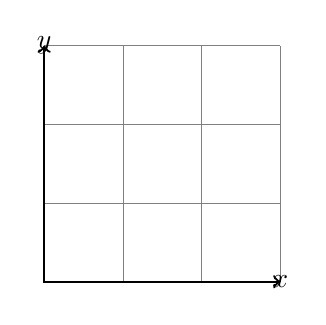
\begin{tikzpicture}
\draw[help lines] (0,0) grid (3,3);
\draw[<->, thick] (0,3) -- (0,0) -- (3,0);
\node (x) at (3,0) {$x$};
\node (y) at (0,3) {$y$};
\end{tikzpicture};

\subsection{How to include Figures}

First you have to upload the image file from your computer using the upload link the project menu. Then use the includegraphics command to include it in your document. Use the figure environment and the caption command to add a number and a caption to your figure. See the code for Figure \ref{fig:frog} in this section for an example.

\begin{figure}
\centering
\includegraphics[width=0.3\textwidth]{frog.jpg}
\caption{\label{fig:frog}This frog was uploaded via the project menu.}
\end{figure}

\subsection{How to add Comments}

Comments \todo{Here is a\\ comment.} can be added to your project by clicking on the comment icon in the toolbar above. % * <john.hammersley@gmail.com> 2016-07-03T09:54:16.211Z:
%
% Here's an example comment!
%
To reply to a comment, simply click the reply button in the lower right corner of the comment, and you can close them when you're done.

Comments can also be added to the margins of the compiled PDF using the todo command\todo{Here's a comment in the margin!}, as shown in the example on the right. You can also add inline comments:

\todo[inline, color=green!40]{This is an inline comment.}

\subsection{How to add Tables}

Use the table and tabular commands for basic tables --- see Table~\ref{tab:widgets}, for example. 

\begin{table}
\centering
\begin{tabular}{|l|c|}
\hline
Item & Quantity \\\hline
Widgets & 42 \\
Gadgets & 13 \\
\hline
\end{tabular}
\caption{\label{tab:widgets}An example table.}
\end{table}

\subsection{How to write Mathematics}

\LaTeX{} is great at typesetting mathematics. Let $X_1, X_2, \ldots, X_n$ be a sequence of independent and identically distributed random variables with $\text{E}[X_i] = \mu$ and $\text{Var}[X_i] = \sigma^2 < \infty$, and let
\[S_n = \frac{X_1 + X_2 + \cdots + X_n}{n}
      = \frac{1}{n}\sum_{i}^{n} X_i\]
denote their mean. Then as $n$ approaches infinity, the random variables $\sqrt{n}(S_n - \mu)$ converge in distribution to a normal $\mathcal{N}(0, \sigma^2)$.


\subsection{How to create Sections and Subsections}

Use section and subsections to organize your document. Simply use the section and subsection buttons in the toolbar to create them, and we'll handle all the formatting and numbering automatically.

\subsection{How to add Lists}

You can make lists with automatic numbering \dots

\begin{enumerate}
\item Like this,
\item and like this.
\end{enumerate}
\dots or bullet points \dots
\begin{itemize}
\item Like this,
\item and like this.
\end{itemize}

\subsection{How to add Citations and a References List}

You can upload a \verb|.bib| file containing your BibTeX entries, created with JabRef; or import your \href{https://www.overleaf.com/blog/184}{Mendeley}, CiteULike or Zotero library as a \verb|.bib| file. You can then cite entries from it, like this: \cite{greenwade93}. Just remember to specify a bibliography style, as well as the filename of the \verb|.bib|.

You can find a \href{https://www.overleaf.com/help/97-how-to-include-a-bibliography-using-bibtex}{video tutorial here} to learn more about BibTeX.

We hope you find Overleaf useful, and please let us know if you have any feedback using the help menu above --- or use the contact form at \url{https://www.overleaf.com/contact}!

\bibliographystyle{alpha}
\bibliography{sample}

\end{document}